\documentclass[12pt]{exam}
\usepackage[T1]{fontenc}
\usepackage[utf8]{inputenc}
\usepackage[brazil]{babel}
\usepackage{lmodern}
\usepackage{graphicx}
\usepackage[normalem]{ulem}
\usepackage{hyperref}

\footer{}{}{}

\title{}
\date{}

\newcommand{\siheader}{
\begin{center}
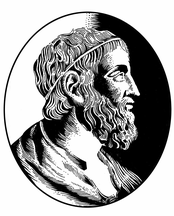
\includegraphics{archi.png}
\vspace{0.5cm}
{\huge Prova de Estágio na Seção de Informática}
\vspace{0.3cm}
\makebox[\textwidth]{Nome:\enspace\hrulefill}
\makebox[\textwidth]{Assinatura:\enspace\hrulefill}
\end{center}
}


\begin{document}
%%% GERAL %%%
\siheader
\section*{Questões}
\begin{questions}

\question
O que é \textit{Software Livre}?
\vfill

\question
O que é uma árvore de diretórios? O que é o diretório raiz?
\vfill

\question
É possível executar programas de Windows no Linux? Justifique.
\vfill

\question
O que é o registro do Windows?
\vfill

\question
Utilizar o pendrive fornecido para \emph{bootar} o computador. Instalar o sistema operacional Linux Mint. Encontrar as informações sobre processador e memória e anotá-las aqui.
\vfill

\question
Configure a rede Eduroam. Tendo conectado à rede, encontrar qual é o IP do computador e o MAC Address da interface de rede utilizada para a conexão. Também anotá-los aqui.
\vfill

\question
Instalar:
\begin{parts}
\part
O IDE Spyder.

\part
O gerenciador de pacotes Pip.

\part
Com o Pip, instalar o pacote \verb+rickroll+.
\end{parts}

\question
Acessar por SSH o servidor shell.ime.usp.br usando as credenciais que forneceremos. Lá:
\begin{parts}
\part
Clonar o repositório: \url{https://github.com/wgnann/estagiosi.git}.

\part
Compilar esta prova, \verb+neoprova.tex+, usando o programa \verb+pdflatex+.
\end{parts}

\end{questions}
\end{document}
